\section{WEB ARAYÜZÜ TASARIMI}

Bu bölümde, Arduino'dan alınan telemetri verilerini gerçek zamanlı olarak polar radar ekranında görselleştiren web arayüzünün tasarımı ve çalışma prensibi açıklanmaktadır.

\subsection{Genel Mimari}

Web arayüzü, üç dosyadan oluşan tek sayfalık bir uygulamadır: \texttt{index.html} (sayfa yapısı), \texttt{styles.css} (görsel tasarım) ve \texttt{app.js} (uygulama mantığı). Arayüz, herhangi bir sunucu veya framework gerektirmeden doğrudan tarayıcıda çalışmaktadır. Kullanıcı, herhangi bir Chrome veya Edge tarayıcısında HTML dosyasını açarak sisteme bağlanabilir.

\subsection{Arayüz Bileşenleri}

Arayüz iki ana bölümden oluşmaktadır:

\begin{itemize}
    \item \textbf{Radar ekranı (sol panel):} HTML5 Canvas elementi üzerine çizilen polar radar görüntüsü. Mesafe halkaları (30, 60, 90, 120, 150~cm), açı çizgileri, tarama çizgisi ve hedef noktaları bu alan üzerinde gösterilmektedir.
    \item \textbf{Kontrol ve bilgi paneli (sağ panel):} Bağlantı durumu, komut butonları (Bağlan, Başlat, Durdur, Simülasyon), anlık ölçüm değerleri (pan, tilt, mesafe, hedef, SD, MPU, ivme, jiroskop, Vcc) ve olay kaydı bölümü.
\end{itemize}

\begin{figure}[!ht]
\centering
	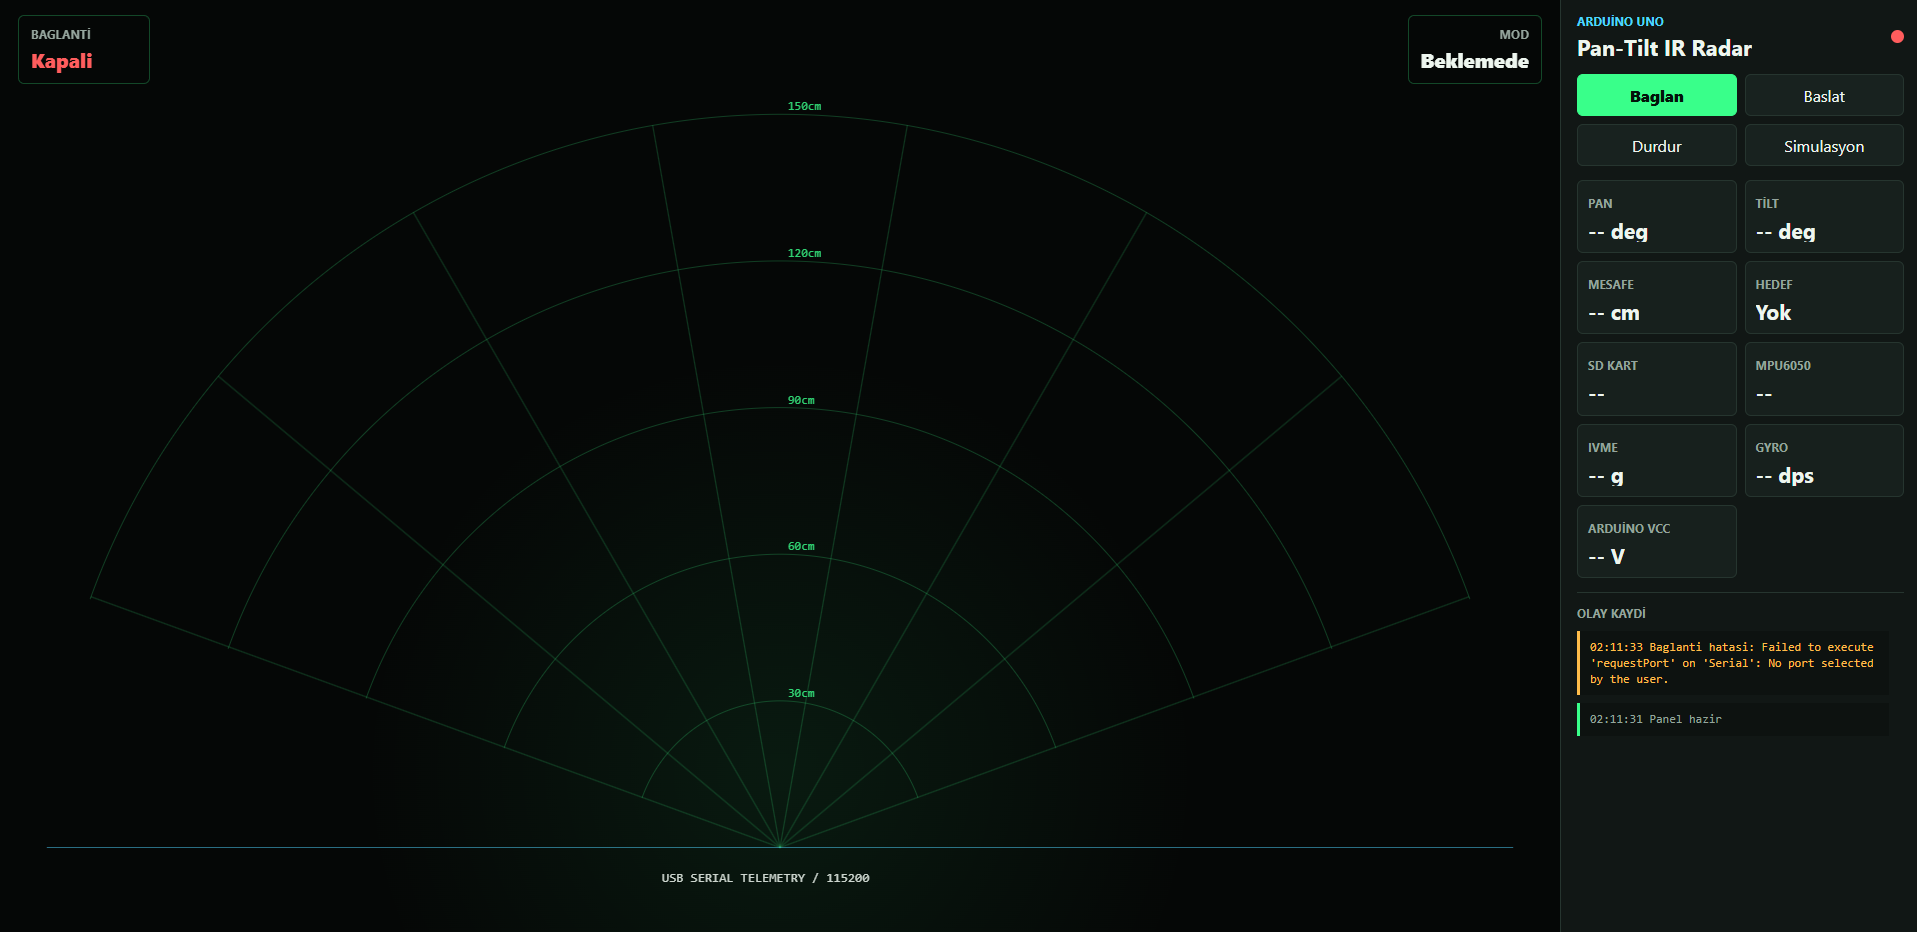
\includegraphics[width=0.85\textwidth]{web_arayuz.png}
	\caption{Web arayüzü genel görünümü}
    \label{fig:web_arayuz}
\end{figure}

\begin{figure}[!ht]
\centering
	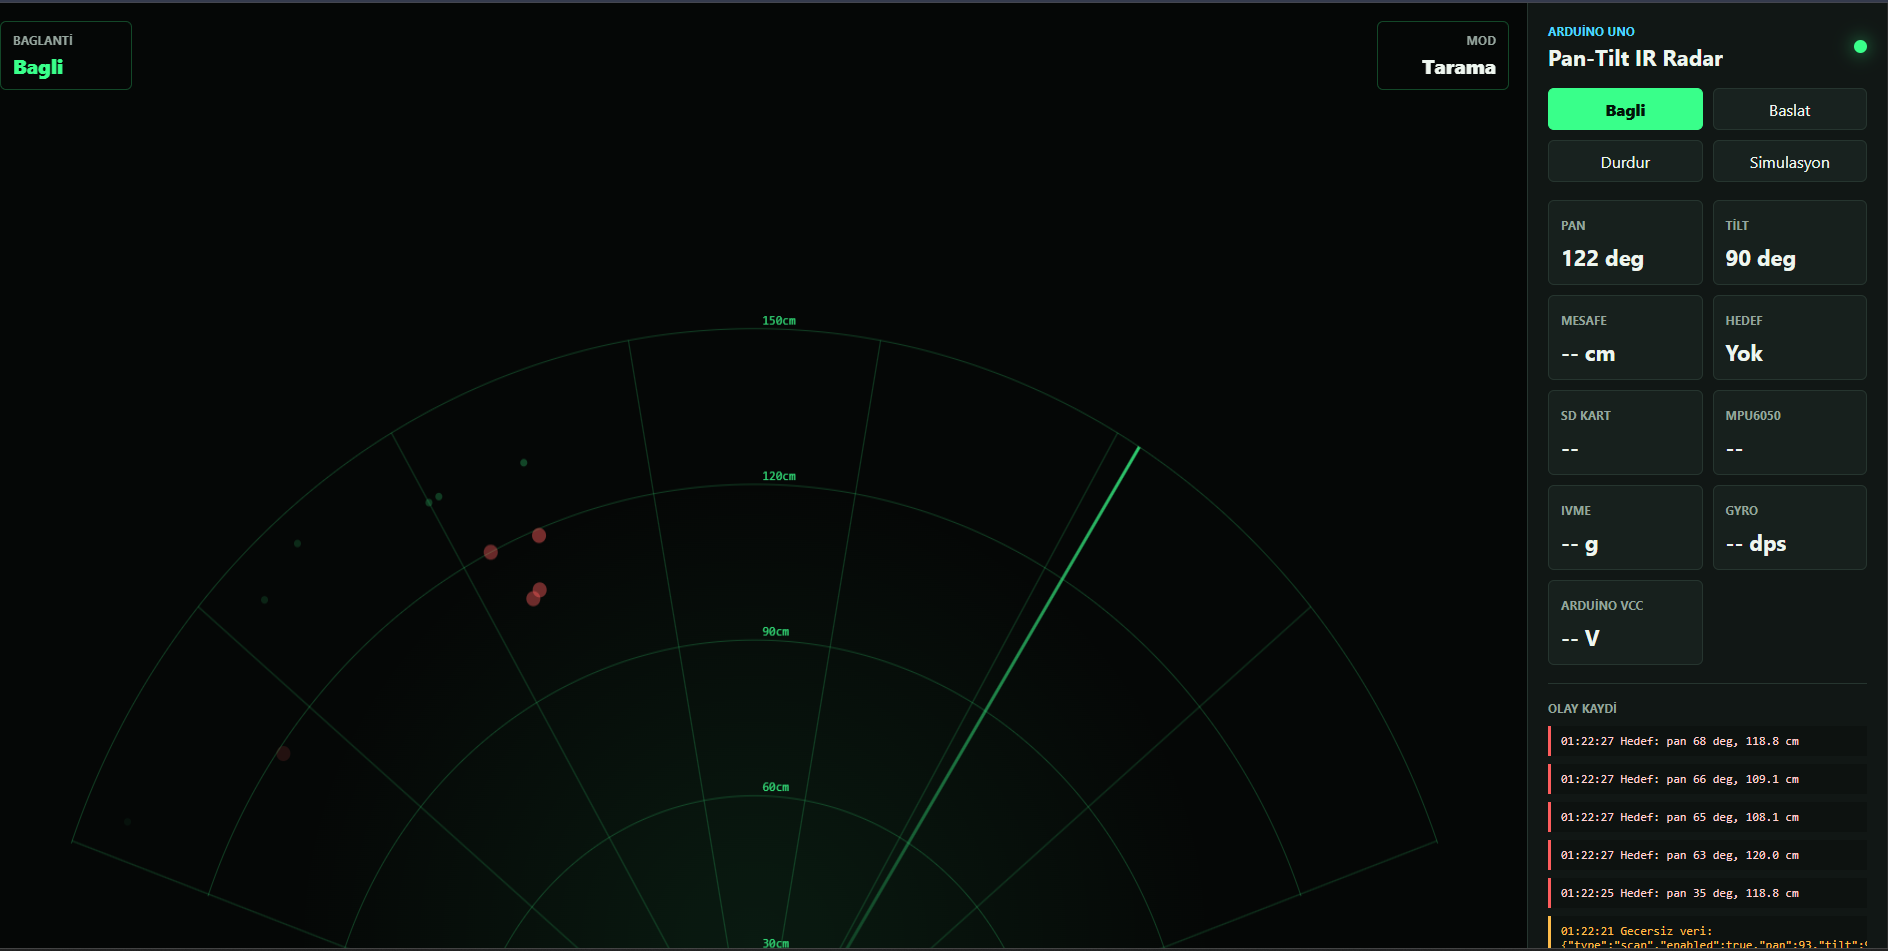
\includegraphics[width=0.85\textwidth]{wearayuz2.png}
	\caption{Web arayüzü -- hedef tespit görünümü}
    \label{fig:web_arayuz2}
\end{figure}

\subsection{Polar Radar Çizimi}

Radar ekranı, \texttt{requestAnimationFrame()} döngüsü ile sürekli yeniden çizilmektedir. Çizim dört aşamadan oluşur:

\begin{enumerate}
    \item \textbf{Izgara çizimi:} 30~cm aralıklarla beş adet mesafe halkası ve $-70$° ile $+70$° arasında 20° aralıklarla açı çizgileri çizilir.
    \item \textbf{Hedef noktaları:} Son 6,5 saniye içinde alınan tarama noktaları çizilir. Her nokta zamanla solarak kaybolur (alpha değeri azalır). Hedef tespit edilen noktalar kırmızı, diğerleri yeşil renkte gösterilir.
    \item \textbf{Tarama çizgisi:} Mevcut pan açısına karşılık gelen doğrusal gradyanlı bir çizgi, radar merkezinden dış kenara doğru çizilir.
    \item \textbf{HUD bilgisi:} Ekranın alt kısmında haberleşme bilgisi gösterilir.
\end{enumerate}

Polar koordinat dönüşümünde pan açısı (20--160°), $-70$° ile $+70$° arasında bir tarama aralığına eşlenir. Mesafe değeri, maksimum mesafeye oranlanarak yarıçap değerine dönüştürülür. Bu iki değer kullanılarak her veri noktasının kartezyen (x, y) konumu hesaplanır.

\subsection{Veri Akışı}

Seri porttan gelen veriler şu adımlarla işlenmektedir:

\begin{enumerate}
    \item Web Serial API ile seri port bağlantısı kurulur (115200~baud).
    \item Gelen byte akışı \texttt{TextDecoder} ile metin dizisine çevrilir.
    \item Satır sonlarına göre ayrıştırılarak her satır bağımsız bir JSON paketi olarak işlenir.
    \item Eksik veya geçersiz JSON paketleri sessizce atlanır; bu durum olay kaydında bildirilir.
    \item Geçerli paketler \texttt{applyPacket()} fonksiyonu ile arayüz elemanlarına yansıtılır.
\end{enumerate}

\subsection{Simülasyon Modu}

Arayüz, Arduino bağlantısı olmadan da test edilebilen yerleşik bir simülasyon moduna sahiptir. Simülasyon modunda JavaScript zamanlayıcısı, 90~ms aralıklarla yapay tarama verileri üretir: pan açısı ileri-geri hareket eder, tilt sinüsoidal salınım yapar ve rastgele hedef noktaları oluşturulur. Bu mod, arayüz geliştirme ve test sürecinde oldukça faydalıdır.
